\chapter{Theoretical Appendix A: Statistical methods and model theory}

\section{Statistical Theory}
\subsection{Bayesian parameter estimation}
\label{ssec:Bayes}
\subsubsection{Problems with frequentist inference using normal models of sample data}
Typical biological practice is to report the mean and variance of a sample, assuming a normal distribution of the error around the mean. In other words, the sample is taken to be representative of a larger population; that population is modelled by a normal distribution with mean $\mu$ and variance $\sigma$; the parameters of the \hyperref[MLE]{maximum likelihood estimate (MLE)} for the normal model are the values reported. A slightly more sophisticated approach is to report the standard error of the mean of the sampling distribution the sample is taken to be drawn from, if more than one sample can be obtained, although this usually plays no role in hypothesis testing (often conducted by t-test).

This approach has a number of defects which follow from one another. We are reporting MLE parameters without any account of our uncertainty about those parameters. There is no way to incorporate prior information we have about the parameters (even just to admit total ignorance about them). This leads to \hyperref[overfit]{overfitting} of our estimates to the sample data. Practically speaking, this means our estimate of the mean is stated too precisely, and the variance is too sensitive to outliers.

Additionally, the plain-sense interpretation of the estimates are often unclear. Means are usually reported plus-minus variance, $\mu\pm\sigma$, and $\sigma$ is often erroneously interpreted as uncertainty about $\mu$ rather than an estimate of a second parameter, the variance of the normal population model. If the frequentist confidence interval for $\mu$ is reported, it is explicitly not understood as the interval in which we have e.g. 95$\%$ confidence that $\mu$ lies, but rather as the interval in which, in the case we repeat the experiment indefinitely, $\mu$ will be found in 95$\%$ of samples. Hypothesis tests are given similarly confusing interpretations involving long-run repeated experiments. These interpretations are widely, if not ubiquitously, misunderstood or ignored in favour of technically incorrect but comprehensible ones \cite{Hoekstra2014, Greenland2016}.

\subsubsection{The Bayesian approach to normal models of unknown mean and variance}
Bayesian methods rectify these problems by understanding the normal model as a model of our information about the population and not of the population itself. This epistemological view of statistics is explicated in \autoref{sec:BayesEpistemology}. Normal gaussian distributions are well-justified both by their ubiquitous success in parameter estimation and by information theoretic considerations \cite{Jaynes2003}, and need not reflect the actual distribution of the population. However, we wish to express our uncertainty about the parameters of a normal gaussian distribution by giving further distributions over the mean $m$ and variance of the normal distribution, with variance usually expressed as precision, $\lambda = 1/\sigma$. Typically, this is done by  assuming normally distributed uncertainty on $\mu$ and gamma distributed uncertainty on $\lambda$, giving rise to a joint normal-gamma (NG) distribution \cite{Bernardo2000}:





An NG distribution may thus serve as a model of our prior information about the population being measured. Because my estimates are the first ones I have made about the relevant populations, and I have no specific guide as to the actual numbers of cells to expect, I have chosen to use the uninformative NG prior:

$p(m,\lambda)$


lies within that range, but is rather understood as the probability that, if the experiment were repeated indefinitely, 95

The appropriateness of the normal model is often in question because it is taken to represent some actually-existing population (which are often not well modelled by normal gaussians). Comparisons of these models using t-tests are given complex interpretations involving long-run rates of error

In Bayesian statistics, available information about a parameter is often modelled by a gaussian distribution over possible values of the parameter. 



\subsection{Bayesian Epistemological View on Model Comparison}




\section{Model Theory}
\subsection{Model optimization}

\subsubsection{MLE}
\label{MLE}

\subsection{Overfitting, Underfitting}
\label{overfit}

\subsection{Monte Carlo simulation}
Referenced on pages: \pageref{TMSmodel}
\label{MonteCarlo}


\subsection{The Akiake Information Criterion For Model Selection}
 
\subsection{Simple Stochastic Models}
\label{SSM}

\begin{figure}
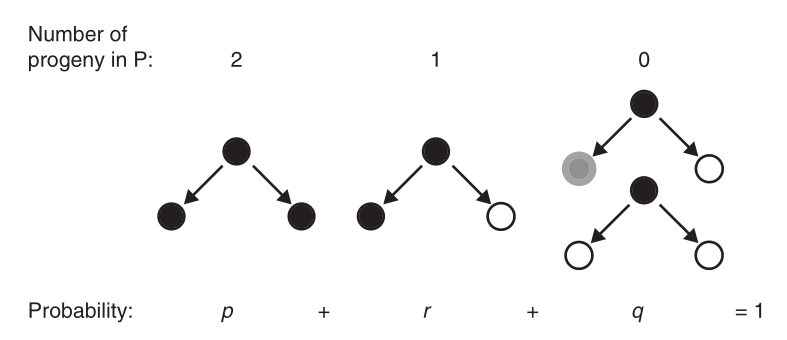
\includegraphics[scale=.5]{simplestochasticmodel}
\centering
\caption{Simple stochastic stem cell model, representing probabilities of cell division events, excerpted from Fagan 2013 pg. 61. Black circles denote proliferative cells, while white and grey circles denote different types of postmitotic offspring. ``Number of progeny in P" is the number of mitotic offspring produced by each type of division. The probability of each division type must sum to 1, as all possibilities are represented, granting that the division types are defined by the postdivisional mitotic history of the offspring.}
\label{fig:SSM}
\end{figure}

The Simple Stochastic Model is schematically summarised in Figure \ref{fig:SSM}. This is the basic structure of the great majority of formal models in the stem cell literature, derived from post-hoc analyses of populations taken to include stem and progenitor cells. The population-level approach is usually explicit, as no differentiation is made between types of proliferating cell- in general, no particular cell is identified with a stem cell, nor can any be identified from the necessarily retrospective population data used to infer the parameters of the model. 

The central concept of the model is that divisions can be categorised by the number of progeny which remain mitotic after the division. It is important to note that a mitotic event cannot presently be categorized in this fashion except retrospectively. This must be kept in mind when analysing models of this type, as this categorisation does not necessarily imply that there is some mechanism by which the cell specifies the fate of offspring \textit{at the time of mitosis}, although there is extensive evidence for the coupling of mitotic and specification processes at the molecular level.

In effect, then, the model compresses the process of fate specification into individual mitotic events. Since the primary distinction between cells in the model is simply whether they are proliferating or not, the model also elides any heterogeneity within the proliferating population. Beyond not identifying particular cells as ``stem cells", this may make models derived from the SSM inappropriate for proliferative populations with a large degree of heterogeneity. One may think here of the classic idea of a small number of slowly proliferating ``true" stem cells and a larger population of rapidly dividing ``transit amplifying" progenitors- this type of internal structure within the proliferating population can only be represented by multiple, independent SSMs (as implemented in \autoref{chap:CMZ}).

As Fagan notes, in the SSM, ``relations among p, r, and q values entail general predictions about cell population size (growth, decrease, or ‘steady-state’), and equations that predict mean and standard deviation in population size, probability of [lineage] extinction, and features of steady-state populations are derived."\footnote{While Fagan refers to ``stem cell" extinction, the model does not specifically define stem cells, nor does it imply intergenerational continuity, such that a particular intergenerationally identified stem cell should be said to have become extinct. The unit which survives or is made extinct is the lineage derived from some particular proliferative cell.}\cite[p.60]{Fagan2013}

Typically, this type of model has been employed to describe population dynamics of proliferating cells in assays generating ostensibly \textit{clonal} data, where a ``clone" here refers to the population constituted by all of the offsping descended from some particular (usually ``initial" and sometimes therefore taken for ``stem") proliferative cell. This population is the \textit{lineage} generated by some particular dividing cell.



\section{Traditional roots of the SMM: Till and McCulloch and the simple stochastic model (SSM)}
\label{TMS}
At the core of the SMM are variants of the most common model used by stem cell biologists, the \hyperref[SSM]{Simple Stochastic Model or SSM}, described in more detail in Section \ref{SSM}. The SSM consists of a Galton-Watson branching process, a stochastic process originally intended to model the lineage extinction of surnames. Wikipedia describes a stochastic process as ``a mathematical object usually defined as a collection of random variables" \cite{Wikipedia2018}. In the case of branching process models applied to proliferative cells, the random variable determines the mode of division of each cell within the lineage, with this mode being defined by the proliferative state (construed in the model as being either mitotic or postmitotic) of progeny. For any given division, a cell may produce two mitotic, one mitotic and one postmitotic, or two postmitotic progeny, and each of these division modes is given a defined (often, but not always, static) probability. Given these values, the history of a cell lineage may be simulated; the output of many of these simulations pooled together, usually by what is referred to as the \hyperref[MonteCarlo]{"Monte Carlo method"}, allows the statistical properties of the dynamics of population of simulated cells to be estimated.

The concept of ``stochasticity" has a long and fraught pedigree in the SCBT. We find it deployed in an identical manner in the early 1960s as today, as in the classic modelling effort of Till, McCulloch, and Siminovitch\footnote{It is worth noting that none of these investigators actually performed the relevant modelling calculations, leaving these to the U of T computer scientist L. Cseh. This division of labour remains lamentably common, and is likely responsible for many of the problems biologists have in understanding the meaning of their mathematical models.} \cite{Till1964}, explaining the variability in the size of ectopic spleen colonies formed by hematopoetic stem cells in irradiated mice by means of a \hyperref[MonteCarlo]{Monte Carlo} \hyperref[SSM]{simple stochastic model (SSM)}. \label{TMSmodel} ``Stochastic" is used in an ambiguous manner here, and, importantly, we find precisely the same ambiguity in Harris' a half century later. This ambiguity arises from the application of the term ``stochastic" to the biological \textit{process} under investigation, to the process' \textit{outcomes}, and to the \textit{model} constructed to describe the process. This is particularly obvious in this early work, entitled ``A Stochastic Model of Stem Cell Proliferation", which states that ``variation [in clonal lineage size] may be generated by a well-known probabilistic (`stochastic') process, the `birth-and-death' process", and that this ``process is operative when an entity, for example, a single cell, may either give rise to progeny like itself (`birth'), or be removed in some way (`death') and these two events occur in a random fashion." \cite{Till1964} As the significance and import of the SMM directly depend on what the meaning of ``stochastic" is, and since the manner in which Harris uses this concept is directly descended from the usage of Till et al., we must sort through this ambiguity before proceeding.

We may clarify the matter by returning to the biological issue at hand, which Till et al. frame in the terms of classic \hyperref[cybernetics]{cybernetic} \label{TMSmodel2} control theory:

\begin{longquote}
[T]he development of a colony involves processes of differentiation occurring among the progeny from a single cell. Analysis of the cell
content of the resulting colony might be expected to cast light on any control
mechanisms which act during colony formation. If rigid control mechanisms are
operative, acting on cells of a relatively constant genotype, all colony-forming cells
might be expected to behave in a similar fashion, and colony formation should be
a relatively uniform process, giving rise to colonies with very similar characteristics.
Alternatively, if control is lax, colonies with widely differing characteristics might
be expected to develop. Results which may bear on this problem are available
from experiments in which colonies were analyzed for their content of colony-
forming cells. It was found that, while most colonies contained these cells,
their distribution among colonies was very heterogeneous, with many colonies
containing few colony-forming cells, and a few containing very many. This result
suggests that control is lax.
\cite{Till1964}
\end{longquote}

This makes quite clear that the essential question here is how the process which produces stem cell proliferative and specificative behaviours is structured. We may think of \hyperref[Waddington]{Waddington's topological model} of cellular specification, itself inspired by \hyperref[cybernetics]{cybernetic theory} \label{TMSmodel3}. Rigid and lax control schemes would, if modelled in this topological fashion, present themselves as very different ``landscapes". The abstract concept At the logical extreme, rigid control of stem behaviour would be represented by a single deep channel, down which the ``ball" (behaving something like a ball bearing) representing ``cellular state" rolls, reliably, at the same rate, in every single instance. Conversely, extremely lax control would be represented by a landscape resembling a Galton board\footnote{The Galton board, named after its inventor, Sir Francis Galton, is significant because the statistical methods Till et al. use to solve the `birth-and-death' process were also invented by him.}, a broad, flat slope with many pegs which may bump the ball this way or that, tending to cluster the balls in the general center of the slope but never preventing some of them from ending up at either extreme (a properly constructed Galton board produces a Gaussian distribution of balls at the bottom of the slope). This metaphor immediately reveals that, \textit{contra} Till et al.'s interpretation of 
